%%% Ne pas modifier jusqu'à la ligne 25
\documentclass[a4paper,12pt]{book}
\usepackage[utf8]{inputenc}
\usepackage[french]{babel}
%%\usepackage{CJK}
\usepackage{yhmath}
\usepackage[left=2cm,right=2cm,top=3cm,bottom=2cm, headheight=1.5cm,headsep=1.5cm]{geometry}
%%\usepackage{CJKutf8}
\usepackage{amsfonts}
\usepackage{amsmath,amsfonts,amssymb,dsfont}
\usepackage{graphicx}
\usepackage{enumitem}		%\enumerate-resume
\usepackage[colorlinks=true,unicode={true},hyperindex=false, linkcolor=blue, urlcolor=blue]{hyperref}
\newcommand{\myref}[1]{\ref{#1} page \pageref{#1}}

\addto\captionsfrench{\def\tablename{Tableau}}  %légendes des tableaux
\renewcommand\thesection{\Roman{section}~-~} 
\renewcommand\thesubsection{\Roman{section}.\Alph{subsection}~-~} 
\renewcommand\thesubsubsection{\Roman{section}.\Alph{subsection}.\arabic{subsubsection}~-~} 

\newcommand{\conclusion}[1]{\newline \centerline{\fbox{#1}}}

\setcounter{secnumdepth}{3}
\parindent=0pt

\usepackage{fancyhdr}
\pagestyle{fancy}

\lhead{SJTU-ParisTech} 
%%%%%%%%%%%%%%%%%%%%%%%%%%%%%%%%%%
\chead{TR5}
\rhead{Daniel 518261910024}

\begin{document}
\renewcommand{\labelitemi}{$\blacktriangleright$}
\renewcommand{\labelitemii}{$\bullet$}


\section{la distance maximale}
\begin{figure}[h]
    \begin{center}
    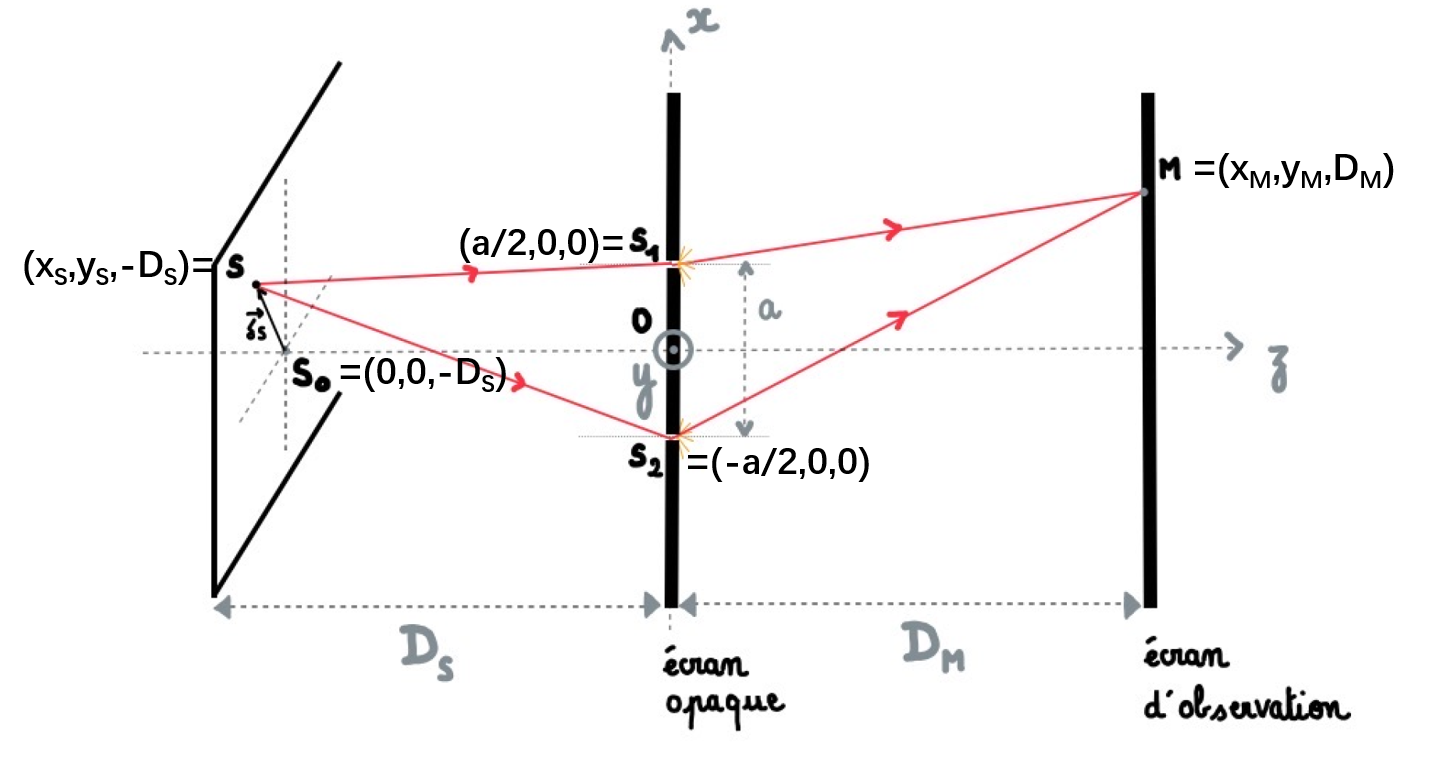
\includegraphics[scale=0.7]{tr5.png}
    \end{center}
    \caption{Expérience des trous de Young}
\end{figure}
On commence par $$\delta_{2/1}(M)=(SM)_2-(SM)_1$$
Supposons que l'expérience est fait dans un milieu homogène d'indice de fraction $n$: 
$(SM)_1=n*SM=n*S_1M+n*SS_1=(S_1M)+(SS_1)$, de même, $(SM)_2=(S_2M)+(SS_2)$, on arrive à 
$$\delta_{2/1}(M)=(SS_2)-(SS_1) + (S_2M)-(S_1M)=SS_2-SS_1 + S_2M-S_1M $$
lorsque on fait l’expérience dans le vide($n=1$). En appliquant les coordonnées, on a 
\begin{align*}
    \delta_{2/1}(M)&=(SS_2-SS_1) + (S_2M-S_1M)\\
                   &=\left(\sqrt{\left(x_s+\frac{a}{2}\right)^2+y_s^2+D_s^2}-
                     \sqrt{\left(x_s-\frac{a}{2}\right)^2+y_s^2+D_s^2}\right)\\
                   &+
                     \left(\sqrt{\left(x_M+\frac{a}{2}\right)^2+y_M^2+D_M^2}-
                     \sqrt{\left(x_M-\frac{a}{2}\right)^2+y_M^2+D_M^2}\right)\\
                   &=D_s\left(\sqrt{\left(\frac{x_s+\frac{a}{2}}{D_s}\right)^2+\left(\frac{y_s}{D_s}\right)^2+1}
                   -\sqrt{\left(\frac{x_s-\frac{a}{2}}{D_s}\right)^2+\left(\frac{y_s}{D_s}\right)^2+1}\right)\\
                   &+D_M\left(\sqrt{\left(\frac{x_M+\frac{a}{2}}{D_M}\right)^2+\left(\frac{y_M}{D_M}\right)^2+1}
                   -\sqrt{\left(\frac{x_M-\frac{a}{2}}{D_M}\right)^2+\left(\frac{y_M}{D_M}\right)^2+1}\right)
\end{align*}
Lorsque l'on fait l'observation au voisinage de l'axe $O_z$ et à grande distance, c'est à dire que 
$|x_s| \ll D_s, |y_s| \ll D_s, |x_M| \ll D_M, |y_M| \ll D_M, |a| \ll D_S, |a| \ll D_M$. 
Donc 
$$
\left(\frac{x_M+\frac{a}{2}}{D_M}\right)^2+\left(\frac{y_M}{D_M}\right)^2\ll 1,\, 
\left(\frac{x_M-\frac{a}{2}}{D_M}\right)^2+\left(\frac{y_M}{D_M}\right)^2\ll 1
$$
et
$$
\left(\frac{x_s+\frac{a}{2}}{D_s}\right)^2+\left(\frac{y_s}{D_s}\right)^2\ll 1,\,
\left(\frac{x_s-\frac{a}{2}}{D_s}\right)^2+\left(\frac{y_s}{D_s}\right)^2\ll 1,\,
$$
Par développement limité à l'ordre 1 que $\sqrt{1+x} = 1+\frac{x}{2}$ lorsque $x\ll 1$, on a 
\begin{align*}
    \delta_{2/1}(M)&=D_s\left(1+\frac{1}{2}\left(\left(\frac{x_s+\frac{a}{2}}{D_s}\right)^2+\left(\frac{y_s}{D_s}\right)^2\right)-1
                 -\frac{1}{2}\left(\left(\frac{x_s-\frac{a}{2}}{D_s}\right)^2+\left(\frac{y_s}{D_s}\right)^2\right)\right)\\
                   &+D_M\left(1+\frac{1}{2}\left(\left(\frac{x_M+\frac{a}{2}}{D_M}\right)^2+\left(\frac{y_M}{D_M}\right)^2\right)-1
                   -\frac{1}{2}\left(\left(\frac{x_M-\frac{a}{2}}{D_M}\right)^2+\left(\frac{y_M}{D_M}\right)^2\right)\right)\\
                   &=D_s\left(\frac{\left(x_s+\frac{a}{2}\right)^2-\left(x_s-\frac{a}{2}\right)^2}{D_s^2}\right)+
                   D_M\left(\frac{\left(x_M+\frac{a}{2}\right)^2-\left(x_M-\frac{a}{2}\right)^2}{D_M^2}\right)
\end{align*}
Finalement, on a $\boxed{\delta_{2/1}(M)=\frac{ax_s}{D_s}+\frac{ax_M}{D_M}}$. 

On a donc le déphasage $\phi_{2/1}(M)=\frac{2\pi}{\lambda_0}\delta_{2/1}(M)=\frac{2\pi}{\lambda_0}\left(\frac{ax_s}{D_s}+\frac{ax_M}{D_M}\right)$

L'éclairement est donc $\boxed{\mathcal{E}(M)=\mathcal{E}_1(M)+\mathcal{E}_2(M)+2\sqrt{\mathcal{E}_1(M)\mathcal{E}_2(M)}\cos\left(\frac{2\pi}{\lambda_0}\left(\frac{ax_s}{D_s}+\frac{ax_M}{D_M}\right)\right)}$

Pour la frange brillante d'ordre 0, il faut que $\frac{2\pi}{\lambda_0}\left(\frac{ax_s}{D_s}+\frac{ax_M}{D_M}\right)=0$, d'où $x_{M,0}=-x_s\frac{D_M}{D_s}$, 
qui a une traslation de $-x_s\frac{D_M}{D_s}$ que $x_{M,0}^{'}=0$(le cas où $S=S_0$). Comme l'interfrange ne change pas, \fbox{tous les franges sont translatées de 
$-x_s\frac{D_M}{D_s}$ selon l'axe $O_x$}.


\end{document}